\chapter{Problèmes difficiles en théorie des nombres}
    \section{Complexité et cryptographie}
        \subsection{Introduction}
            Idée : mesurer la "difficulté" algorithmique d'un problème.
            \begin{defi} (Problème de décision)
                Un problème de décision est une collection d'instances qui sont des ensembles de données qui admettent exactement une des deux réponses "oui" ou "non".
            \end{defi}
            \begin{expl}
                \begin{enumerate}
                    \item Problème SAT (Satisfaisabilité) 
                    \begin{description}
                        \item[Instance :] Une fonction à variables booléenne $F : \{0,1\}^n \to \{0, 1\}$ construite avec les connecteurs logiques $\lor, \land, \lnot$. Par exemple,
                        \begin{align*}
                            f(x_1, x_2, x_3, x_4) = (\lnot (x_1 \land (\lnot x_3))) \lor (x_1 \land x_2 \land (\lnot x_1))
                        \end{align*}
                        \item[Question :] existe-t-il $x_1, \cdots, x_n \in \{0, 1\}$ temls que $F(x_1, \cdots, x_n) = 1$ ?
                        \item[Algorithme :] recherche exhaustive sur $(x_1, \cdots, x_n)$, la complexité est en $\mathcal{O}(2^n)$.
                    \end{description}
                    \item FBQ (Formes Booléennes Quantifiées)
                    \begin{description}
                        \item[Instance :] Une formule booléenne avec quantificateur e.g. $\forall x_i \exists x_j \cdots F(x_1, \cdots, x_n)$ ($F$ est une fonction booléenne comme dans SAT)
                        \item[Question :] Cette formule est-elle vraie ? 
                        \item[Algorithme :] Recherche exhaustive ($\mathcal{O}(2^n)$).  
                    \end{description}
                    \item Equations diophantiennes ($10^\text{ème}$ problème de Hilbert)
                    \begin{description}
                        \item[Instance :] Une équation polynomiale à plusieurs inconnues et à coefficients entiers
                        \item[Question :] Cette équation admet-elle des solutions entières ?
                        \item[Algorithme :] Matyasevich, 1971 : il n'y a pas d'algo qui répond à cette question.  
                    \end{description}
                \end{enumerate}
            \end{expl}

        \subsection{Calculabilité au sens de Turing}
            Turing : Cryptanalyse d'Enigma, construction de machines dédiées à la cryptanalyse d'Enigma, Machine de Turing.
            
            \subsubsection{Modèle de Turing}
                On dispose d'un ruban infini
                \begin{figure}[H]
                    \centering
                    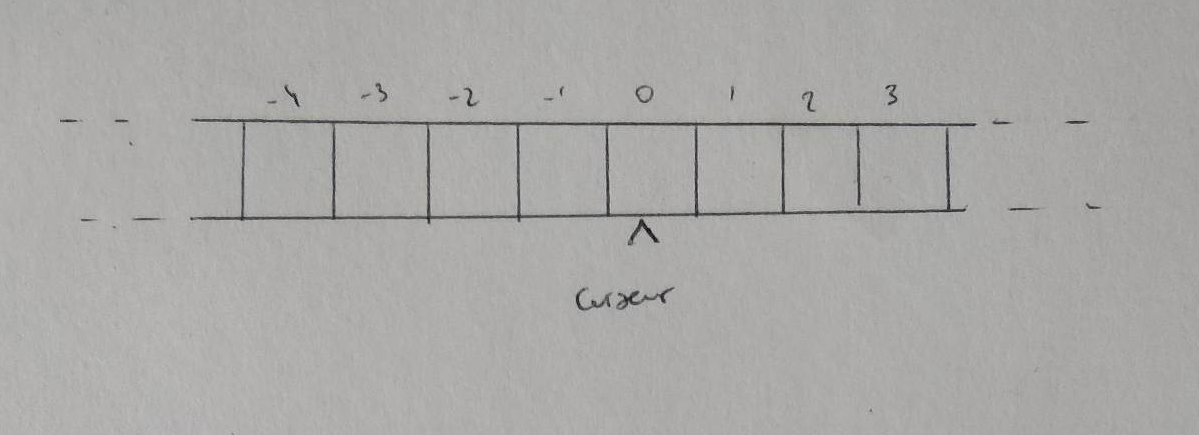
\includegraphics[width=.5\textwidth]{01}
                \end{figure}
                Chaque case contient un symbôle (dans un alphabet fini $\Sigma$ que l'on peut supposer être $\{0, 1\}$, ou le symbôle blanc $b$). Le ruban v aêtre lu case par case par le curseur, la machine est à chaque instant dans un état $q_i \in Q$, où $Q$ est l'ensemble fini des états possibles.
                \begin{defi} (Machine de Turing)
                    Une opération élémentaire est entièrement déterminée par le symbôle lu par le curseur, et par l'état actuel $q_i$ :
                    \begin{enumerate}
                        \item Le curseur remplace le symbôle par un élément de $\Sigma \cup \{b\}$
                        \item Le curseur de déplae soit d'une case vers la gauche, soit d'une case vers la droiten, soit reste sur place.
                        \item La machine passe de l'état $q_i$ à l'état $q_j$.
                    \end{enumerate}
                    Une machine de Turing est donc la donnée d'une fonction
                    \begin{align*}
                        M : (\Sigma \cup \{b\}) \times Q \to (\Sigma \cup \{b\}) \times \{-1, 0, 1\} \times Q
                    \end{align*}
                \end{defi}
                \begin{defi} (Calcul déterministe)
                    Le calcul déterministe d'une entrée $x$ avec une machine de Turing $M$ est la suite d'opération suivante :
                    \begin{enumerate}
                        \item La machine est commence par être dans l'état $q_0$
                        \item Le curseur est placé sur la case $1$
                        \item $x$ est écrite sur les cases $1, \cdots, n$ du ruban, les autres contenant $b$.
                        \item On applique itérativement $M$, le calcul se terine lorsque la machine atteint l'état final $q_F$. La sortie $y$ est alors la donnée inscrite sur le ruban lorsque la machine termine.
                    \end{enumerate}
                \end{defi}
                Terminologie : L'ensemble des suites finies de symbôles de $\Sigma$ est noté $\Sigma^*$. Un mot est un élément de $\Sigma^*$. Une fonction $f : \Sigma^* \to \Sigma^*$ est turing calculable s'il existe une machine de Turing $M$ qui sur tout entrée $x \in \Sigma^*$ calcule $y = f(x)$.

        \subsection{Complexités en temps et classes $P$, $NP$}
            \begin{defi}
                La longeuru d'un calcul sur une entrée $x \in \Sigma^*$ pour une machine de Turing $M$ est le nombre $t_M(x)$ d'opération élémentaires qui composent le calcul. Ainsi on défini la complexité en temps d'une machine de Turing comme
                \begin{align*}
                    \begin{array}{cccc}
                        T_M : & \mathbb{N} & \to & \mathbb{N} \\
                        & n & \mapsto & \max_{\substack{x \in \Sigma^* \\ |x| = n}} \{t_M(x)\} \\
                    \end{array}
                \end{align*}
            \end{defi}
            \begin{defi}
                Un algorithme polynomial $\mathcal{A}$ pour calculer $f$ est une machine de Turing $M$ qui calcule $f$ et telle qu'il existe un polynôme $p$ tel que $\forall n \in \mathbb{N}$, $T_M(n) \leq p(n)$. On appelle classe $P$ l'ensemble des problèmes de décision admettant un algorithme polynomial.
            \end{defi}
            \begin{defi}
                On dit qu'un pb de décision est calculable par un algo non déterministe polynomial s'il existe une machien de Turing $M$ et un polynome $p$ tel que 
                \begin{enumerate}
                    \item La réponse est oui pour l'entrée $x$ ssi il existe $y \in \Sigma^*$ (certificat) tel que $M$ calcule $1$ lorsqu'on met $x \in \Sigma^*$ dans les cases $1$ à $n$ et $y$ dans les cases $-1$ a $-m$.
                    \item Pour tout $x$ donnant la réponse $1$, $M$ calcule $1$ et temps $\leq p(n)$
                \end{enumerate}
                On appelle classe $NP$ la classe des problèmes de décision admettant un algorithme non déterministe polynomial.
            \end{defi}
            \begin{remq}
                $P \subseteq NP$.
            \end{remq}
            
        \subsection{Problèmes $NP$-complets}
            \begin{defi}
                On dit que le problème de décision $p_1$ se réduit au problème de décision $p_2$ s'il existe une fonction $\varphi : \Sigma^* \to \Sigma^*$ calculable en temps polynomial telle que la réponse à $p_1$ est oui pour l'entrée $x$ si et seulement si la réponse à $p_2$ est oui pour l'entrée $\varphi(x)$.
            \end{defi}
            \begin{nota}
                On note $p_1 \ltimes p_2$.
            \end{nota}
            \begin{prop}
                $p_1 \in P$ et $p_1\ltimes p_2 \Rightarrow p_1 \in P$
            \end{prop}
            \begin{defi}
                Un problème $\Pi$ est $NP$-complet ssi $\forall p \in NP$, $p \ltimes \Pi$.
            \end{defi}
            \begin{theo} (Cook, 1971)
                SAT est $NP$-complet.
            \end{theo}
            \begin{remq}
                Si $SAT \ltimes P$, alors $P$ est $NP$-complet.
            \end{remq}
            \begin{expl}
                \begin{enumerate}
                    \item SAT
                    \item $3$-SAT
                    \item Circuit hamiltonien
                    \item $3$-coloriabilité d'un graphe
                    \item TSP
                    \item Pb du sac à dos
                    \item Système de $n$ équations quadratiques sur un $\mathbb{F}_2$.
                \end{enumerate}
            \end{expl}
            On conjecture que $P \neq NP$. Astuce de Levin : Supposons que $P = NP$ : alors on peut construire un algorithme polynomial pour résoudre $SAT$. Considérons les machines de Turing $M_1, M_2, \cdots$ qui prennent en entrée une instance de $SAT$ : Alors on fait tourner les machines simultanément, en faisant tourner de une étape $M_1$, puis en faisant tourner de une étape $M_2$, puis $M_1$, puis $M_3$, $M_2$ et $M_1$, etc. 

            \subsubsection{Résumé de la hiérarchie des complexités algorithmiques :}
                \begin{figure}[H]
                    \centering
                    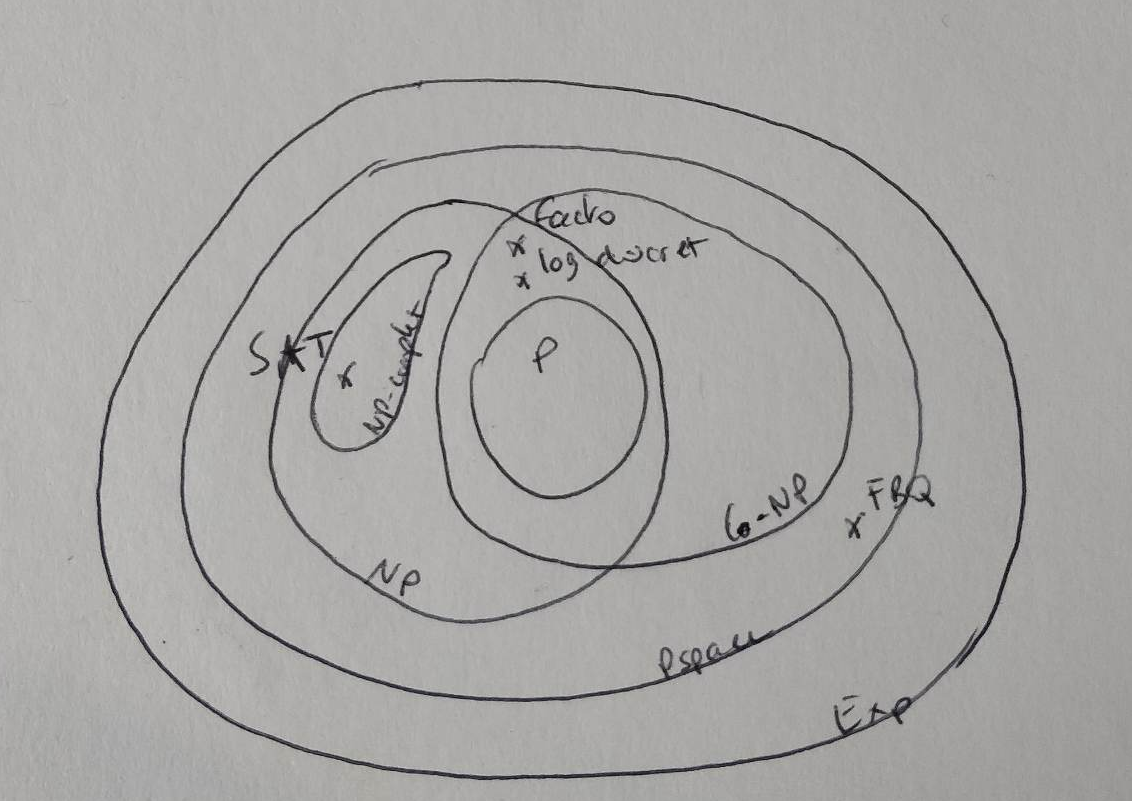
\includegraphics[width=.5\textwidth]{02}
                \end{figure}
                \begin{remq}
                    Co-$NP \cap NP$-complet $= \emptyset$.
                \end{remq}

    \section{Factorisation}
        \subsection{Complexité}
            Problème de décision FACTM (problème des facteurs majorés)
            \begin{itemize}
                \item Instance : $n$ entier, $M \leq n$.
                \item Question : Existe-t-iil un diviseur de $n$ qui est $\leq M$.
            \end{itemize}
            Si on a un algo polynomial de factorisation, alors on peut résoudre FACTM en temps polynomial. Inversement, Supposons $\mathcal{A}$ algo polynomial pour FACTM. Comment factoriser $n$ ? Soit $p$ le plus petit facteur premier de $n$, alors
            \begin{itemize}
                \item On applique $\mathcal{A}(n, \sqrt{n})$. Si l'algorithme répond non, alors on termine et on répond non (car $n$ est alors premier)
                \item Sinon, on applique $\mathcal{A}(n, \sqrt{n}/2)$. Si l'algo répond non, alors $p \in [\sqrt{n}/2, \sqrt{n}]$, et sinon $p \in [1, \sqrt{n}/2]$.
                \item On continue la dichotomie jusqu'à ce que la taille de l'intervalle obtenu soit plus petite que $1$.
            \end{itemize}
            L'algorithme termine dès que $\sqrt{n}/2^k <1$, où $k$ est le nombre d'appels de $\mathcal{A}$. Ainsi il y a $k = \log_2(\sqrt{n})$ est donc de l'ordre de $\log n$. Une fois $p$ trouvé, on recommence l'algo avec $n/p$. On va recommencer le nombre de facteurs premiers de $n$ (comptés avec leur multiplicité). Mais
            \begin{align*}
                n = \prod_i p_i^{\alpha_i} \geq \prod_i 2^{\alpha_i} = 2^{\sum \alpha_i}
            \end{align*}
            donc $\sum \alpha_i < \log_2 n$, et c'est aussi le nombre de facteurs premiers de $n$ (comptés avec leur multiplicité). Au total, l'algorithme est polynomial.

        \subsection{Idée de Fermat}
            \begin{itemize}
                \item L'idée naïve est d'essayer de diviser par les entiers successifs $\leq n$. C'est en $\mathcal{O}(n)$ donc exponentiel en la taille de l'entier.
                \item On peut aussi s'arrêter avant $\sqrt{n}$, mais l'algorithme reste exponentiel.
                \item On peut aussi diviser par les nombres premiers $\sqrt{n}$. D'après le théorème des nombres premiers (Hadamard, de la Vallée-Poussin), le cardinal des entiers premiers plus petits que $x$ est aymptotiquement équivalent à $x/\ln x$. Ainsi l'algo est en $\mathcal{O}(\sqrt{n}/\log n)$, qui reste exponentiel en la taille de $n$.
            \end{itemize}
            Il suffit, pour factoriser $n$, de trouver $x$ et $y$ tels que $x^2 = y^2 [n]$, avec $x \neq \pm y [n]$. En effetn on a alors $(x - y)(x + y) = 0 [n]$ et ainsi $\gcd (x, x-y)$ est un facteur de $n$. Fermat prend comme valeurs de $x$ $\lfloor \sqrt{n} \rfloor + 1, \lfloor \sqrt{n} \rfloor + 2$, et espère que $x^2 - n$ est un carré parfait $y^2$. SAUCISSE. 
            \begin{expl}
                $n = 9167$, $\sqrt{n} = 95,7$, $96^2 = 49 [n]$, et $49 = 7^2$, et alors $\gcd (9167, 96+7) = 103$, $\gcd (9167, 96 - 7) = 89$. On a bien $9167 = 103 \times 89$.
            \end{expl} \noindent
            La complexité est de l'ordre de $\sqrt{n}$, c'est donc toujours exponentiel. Donnons un rafinement de la méthode : prenons $n = 849239$, $\sqrt{n} = 921,5$.
            \begin{itemize}
                \item $922^2 = 845 = 5 \times 13^2 [n]$
                \item $933^2 = 2 \times 5^4 \times 17 [n]$
                \item $937^2 = 2 \times 5 \times 13^2 \times 17 [n]$
            \end{itemize}
            Et alors $(922 \times 933 \times 937)^2 = (2 \times 5^3 \times 13 \times 17)^2 [n]$ et donc on a trouvé l'équation qu'on voulait, et après calcul des pgcd on obtiens que $1229 \times 691 = 849239$. On vient de décrire le crible quadratique de Pomerance. 
            
            \subsubsection{Algorithmes} 
                Décrivons le dans sa généralité : on veut factoriser $n$, pour cela
                \begin{enumerate}
                    \item On se fixe une base de factorisation $B = \{-1, p_1, p_2, \cdots, p_h\}$. 
                    \item On dit qu'un entier est friable (ou lisse/smooth) s'il n'a que des petits facteurs premiers. Précisément, il est $B$-friable si tous des facteurs premiers sont dans $B$.
                    \item On va dire que $b$ est $B$-adapté si le représentant de $b^2[n]$ dans l'intervalle $[-n/2, n/2]$ est $B$-friable. 
                \end{enumerate}
                \begin{description}
                    \item[Etape 1 :] Obtenir et stocker des entiers $b_i$ qui sont $B$-adaptés. On note
                    \begin{align}
                        \label{relation}
                        b_i^2 = (-1)^{\varepsilon_i} p_1^{\alpha_{i,1}} \cdots p_h^{\alpha_{i,h}} [n]
                    \end{align}
                    \item[Etape 2 :] A chaque relation  \ref{relation}, on associe 
                    \begin{align*}
                        u_i = (u_{i, 0}, \cdots, u_{i,h}) \in \mathbb{F}_2^{h + 1}
                    \end{align*}
                    où $u_0 = \varepsilon_i [2]$, $u_{i,j} = \alpha_{i,j} [2]$ si $j \geq 1$.
                    \item[Etape 3 : ] on a
                    \begin{align*}
                        \Rightarrow \prod_{i \in I} (b_i^2)^{\beta_i} &= \prod_{i \in I} \left( (-1)^{\varepsilon_i} \prod_{j = 1}^h p_j^{\alpha_{i,j}} \right)^{\beta_i} [n] \\
                        &= (-1)^{\sum_{i \in I} \beta_i \varepsilon_i} \times \prod_{j = 1}^h p_j^{\sum_{i \in I} \beta_i \alpha_{i, j}} [n]
                    \end{align*}
                    donc si on trouve une combinaison linéaire des $u_i$ qui est nulle
                    \begin{align*}
                        \sum_{i \in I} \beta_i u_i = 0
                    \end{align*}
                    les exposants dans la dernière ligne du calcul sont pairs. On a donc $x^2 = y^2 [n]$, avec 
                    \begin{align*}
                        &x := \prod_{i \in I} b_i^{\beta_i} ,\, y = \prod_{j = 1}^h p_j^{\frac12 \sum \beta_i \alpha_{i,j}}
                    \end{align*}
                \end{description}

            \subsubsection{Complexité de l'algorithme}
                \begin{description}
                    \item[Etape 2 :]  Il faut $|I| \geq h + 2$.
                    \item[Etape 1 :] Pour évaluer la complexité de l'étape 1, on utilise
                    \begin{theo}
                        On pose
                        \begin{align*}
                            \psi(x, T) = \card{\{n \leq x \mid n \text{ a tous se facteurs premiers } \leq T\}}
                        \end{align*}
                        Pour $1 \leq T \leq x$, on pose $v := \frac{\ln x}{\ln T}$, alors
                        \begin{align*}
                            \frac{\psi(x, T)}x = v^{-v + o(1)}
                        \end{align*}
                    \end{theo}
                    On prend $B = \{-1, p_1, \cdots, p_h\}$, avec $p_1, \cdots, p_h$ les entiers premiers qui sont $\leq T = \mathrm{exp}\left(\frac12 \sqrt{\ln n \ln \ln n}\right)$. Alors 
                    \begin{align*}
                        v = \frac{\ln \sqrt{n}}{\ln T} = \frac{\frac12 \ln n}{\frac12 \sqrt{\ln n \ln \ln n}} = \sqrt{\frac{\ln n}{\ln \ln n}}
                    \end{align*}
                    donc $\ln v \simeq \frac12 \ln \ln n$. Ainsi le nombre de valeurs à essayer dans la première étape est $(h  + 2)v^v$. Et
                    \begin{align*}
                        v^v = \e^{v \ln v} = \e^{\frac12 \sqrt{\ln n \ln \ln n}} = T
                    \end{align*}
                    Ainsi le nombre d'essais vaut $T(h + 2)$, et $h + 2 \sim T/\ln T$.
                    \item[Etape 3 :] Finalement, la complexité de l'algorithme complet  vaut 
                    \begin{align*}
                        \frac{T^2}{\ln T} + (h + 2)^3 \sim \left( \frac{T}{\ln T} \right)^3 = \e^{\frac32 \sqrt{\ln n \ln \ln n}}
                    \end{align*}
                    On vient donc de décrire un algorithme sous-exponentiel.
                \end{description}
                \begin{nota}
                    \begin{align*}
                        L_{\alpha, c}(z) = \e^{c (\ln Z)^\alpha (\ln \ln z)^{1 - \alpha}}
                    \end{align*}
                    \begin{itemize}
                        \item $\alpha = 0$ : alors $L_{0, c}(z) = \e^{c \ln \ln z} = (\ln z)^c$ donc complexité polynomiale.
                        \item $\alpha = 1$ : $L_{1, c}(z) = \e^{c \ln z}$ donc complexité exponentielle.
                        \item $0 \leq \alpha \leq 1$, alors $L_{\alpha, c}(z)$ est sous-exponentiel.
                    \end{itemize}
                \end{nota}
                Dans le cas de l'algorithme que l'on vient de décrire, la complexité vaut $L_{\frac 12, c}$. Actuellement, le meilleur algorithme pour des nombres types clés de RSA est GNFS (General Number Field Sieve) dont la complexité est $L_{\frac13, c}(n)$ avec $c = 1,92$ (algorithme du à H. Lenstra, A. Lenstra, Manasse, Pollard, 1990).
                \begin{remq}
                    Si on veut $L_{\frac13, c}(n) \geq 2^{80}$, il faut prendre $|n| = 1024$ bits.
                \end{remq}
                \begin{remq}
                    L'exposant $3$ qui vient du pivot de gauss (3eme étape) peut être amélioré : le système à résoudre est un système creux :
                    \begin{align*}
                        b_i^2 = \prod_{j = 1}^h p_j^{\alpha_{i, j}} [n]
                    \end{align*}
                    Le nombre de facteurs premiers qui interviennent dans cette décomposition est de l'ordre $\mathcal{O}(\ln n)$. Ainsi les lignes du système à résoudre contiennent beacoup de zéros, et il existe un algorithme (Block-Lanczos) pour ce genre de système qui est en $\mathcal{O}(dh^2)$ où $h$ est la dimension du système et $d$ est le nombre macimal d'éléments non nuls dans chaque ligne.
                \end{remq}

    \section{Logarithme discret}
        \subsection{Complexité}
            Problème du log discret : soit $p$ un nombre premier, $g$ un générateur de $\znz{p}^*$. À partir de $y = g^x [p]$, retrouver $x$ ? On peut lui associer le problème de décision suivant :
            \begin{description}
                \item[Instance :] $p, g, y, t$
                \item[Question :] Le log discret de $y$ par rapport à $g$ est-il $\leq t$ ? 
            \end{description}
            Si on a un algo $A$ polynomial pour le problème de décision, alors de manière similaire au problème de factorisation (dichotomie), on peut calculer le log discret en temps polynomial.

        \subsection{Méthodes de calcul du log discret}
            \begin{itemize}
                \item Méthode naïve : recherce exhaustive sur $x$, complexité en $\mathcal{O}(p)$ (donc exponentiel).
                \item Méthode baby step giant step : On regarde la division euclidienne de $x$ par $a$ où $a = \lfloor \sqrt{n} \rfloor$. Trouver $x$ est équivalent à trouver $q, r$ et poser $x = aq + r$. Maintenant 
                \begin{align*}
                    y = g^x [p] \iff yg^{-aq} = g^r[p]
                \end{align*}
                On peut créer 2 tables de $0$ à $a$ indexées par $q$ et $r$ où on calcule $yg^{-aq}$ et $g^r$, et on cherche une valeur commune. Si les tables sont triées, alors la recherche d'une valeur commune est en $\mathcal{O}(a)$. 
            \end{itemize}
            
        \subsection{Méthode du calcul d'indices}
            On cherche $x$ tel que $g^x = y[p]$.
            \begin{description}
                \item[ $\emptyset$ Etape 1 :] On choisit $B = \{-1, p_1, \cdots, p_h\}$
                \begin{itemize}
                    \item On choisit $c_i$ aléatoire
                    \item On calcule le représentant de $g^{c_i}[p]$ dans $[-p/2, p/2]$ et on espère que $g^{c_i}[p] = \prod_{j = 0}^h p_j^{\alpha_{i,j}} \, (*)$, dans ce cas on aura $c_i = \sum_{j = 0}^h \alpha_{i,j} \log_g(p_j) [p_1]$.
                \end{itemize} 
                \item[1Etape 2 :] Si on a obtenu $\geq h + 1$ relations du type $(*)$, on pourra trouver les $\log_g(p_j)$ pour $0 \leq j \leq h$.
                \item[Etape 3 :] On calcule $yg^e [p]$ où $e$ est aléatoire. Avec une certaine probabilité, $yg^e = \prod_{j = 0}^h p_j^{\beta_j}$, et alors
                \begin{align*}
                    \log_g(y) = \left(\sum_{j = 0}^h \beta_j \log_h(p_j)\right) - e
                \end{align*}
            \end{description}
            Par un argument similaire à l'analyse de complexité de l'algorithme de factorisation, on obtiens une complexité en $\mathcal{O}(\e^{1 + o(1) \sqrt{\ln p \ln \ln p}})$, doit du $\mathcal{O}(L_{\frac12, 1 + o(1)}(p))$. Le meilleur algorithme est en $L_{\frac13, c}$ avec $c = 1,92$. 